\documentclass[../main.tex]{subfiles}
\begin{document}

\section{Monsters}
There are two types of Lost Monsters in TimeStrike: Beasts and Brutes. These Monsters are summoned throughout the game, slowly becoming an ever-greater threat to the players’ Characters. Sentience cards will frequently cause Monsters to attack non-Lost units. Monsters can be attacked, tamed, or defeated.

\subsection{Beasts}
A Beast is a small type of Lost Monster in TimeStrike. Beasts start on the board and more are summoned throughout the game. Beasts can be attacked for loot, tamed, or defeated.

\subsection{Brutes}
A Brute is a large multi-hex type of Lost Monster. Brutes are summoned throughout the game onto the board. Brutes can be attacked for loot, tamed, or defeated. Brutes are highly valuable Monsters that can be tamed and then mounted by Survivors to create unique and powerful Character combinations.

\subsection{Taming}
Taming is a mechanic used to capture and recruit Monsters to a team. Beasts and Brutes can be tamed by Survivor units. Tamed Monsters can then be activated when taking a turn with the Character that tamed them.

\textit{Note: Tamed Monster are no longer considered Lost units.}

\subsubsection{Tamed Beasts}
When a Beast is tamed, its Character card is placed next to the Character card of the unit that tamed it. When taking a turn with a Character that has tamed one or more Beasts, you may also activate each Beast the Character has tamed. If a Character that tamed one or more Beasts is defeated, each tamed Beast will revert to a Lost unit controlled by the Sentience.
\begin{figure}[h]
    \centering
    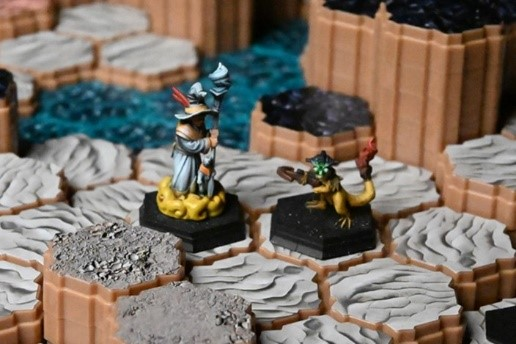
\includegraphics[width=1\linewidth]{chapters//Monsters/TimeStrikeTamedBeasts.jpg}
\end{figure}

Image: Character with a tamed Beast. 

\subsubsection{Tamed Brutes}
When a Brute is tamed, the unit that tamed it is mounted on top of it. The two units are collectively called a Behemoth. When taking a turn with a Character that has tamed one or more Brutes, you may also activate each Brute the Character has tamed. When activating a unit mounted on a Brute, it may no longer use its Movement stat, but still uses its own Energy to perform actions.

\begin{figure}[h]
    \centering
    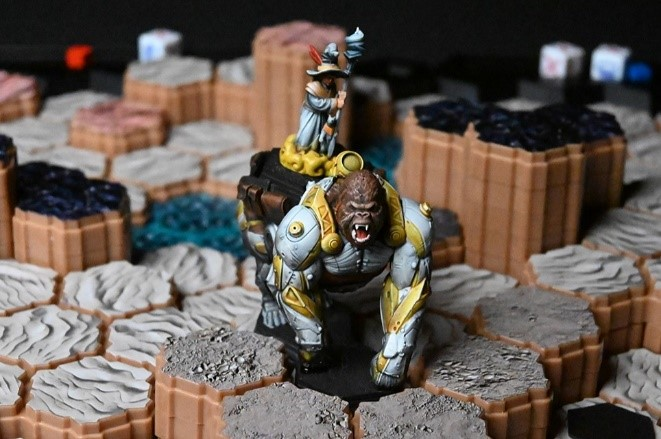
\includegraphics[width=1\linewidth]{chapters//Monsters/TimeStrikeTamedBrute.jpg}
\end{figure}

\subsubsection{Behemoths}
Units mounted on tamed Brutes cannot be targeted by enemies.

If a tamed Brute is targeted for an attack and receives any damage from the attack, the mounted unit must also roll Defense against each attack icon from that attack.

If a tamed Brute is defeated, the mounted unit is placed by its owner on any unoccupied hex that the Brute previously occupied.

If a mounted unit is defeated, the Brute reverts to a Lost unit controlled by the Sentience.

\subsection{Monster Targeting System}
When a Monster is required to acquire a target on its own, the Monster will first attempt to target the closest player unit within range without moving. If there is no targetable unit within range, it will then start to move in the direction of the nearest hex from which it could target a player unit. If the Monster cannot reach a hex from which it could target a player unit, it will spend all its Movement attempting to get as close as possible to that hex.

\textit{Note: If more than one player unit is an equal targetable distance away, players will roll D20s to determine which unit the Monster will attempt to target; the Monster will attempt to target the unit with the lowest roll.}

\clearpage
\end{document}